\documentclass[12pt]{article}

\title{Using idiolects to improve word prediction}
\author{Wessel Stoop}

\usepackage{covington}
\usepackage{graphicx}
\usepackage{float}
\usepackage{apacite}
\usepackage{qtree}

%Set font
\renewcommand{\familydefault}{\sfdefault}

%Tables captions small
\usepackage{caption3} % load caption package kernel first
\DeclareCaptionOption{parskip}[]{} % disable "parskip" caption option
\usepackage[footnotesize]{caption}

%Line spacing
\linespread{1.5}

%New page for every chapter
\let\stdsection\section
\renewcommand\section{\newpage\stdsection}

%Center tables
\let\originaltable\table
\let\endoriginaltable\endtable
\renewenvironment{table}[1][ht]{%
  \originaltable[#1]
  \centering}%
  {\endoriginaltable}

\begin{document}

\begin{table}[b]
\begin{tabular}{ll}
\textbf{Master's thesis}&\\
Name&Wessel Stoop\\
Student numbers&s0808709 (Nijmegen), u1249664 (Tilburg)\\
Supervisor&Antal van den Bosch\\
Period&Spring 2013\\
\end{tabular}
\end{table}

\maketitle
\thispagestyle{empty}

\begin{figure}
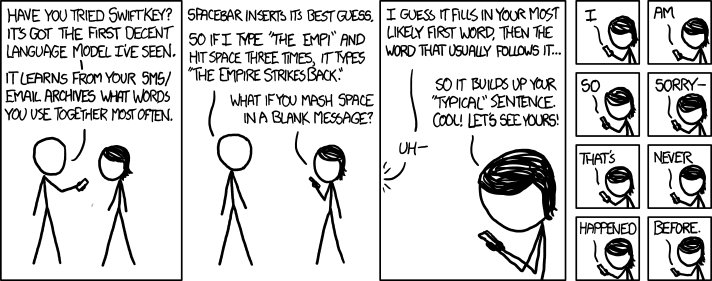
\includegraphics[scale=0.5]{swiftkey}
\end{figure}

\clearpage

\tableofcontents
\listoftables
\listoffigures

\section{Summary/samenvatting}

\subsection{English}
In this thesis, the word prediction system \emph{Soothsayer} is described. This system predicts what a user is going to write as he/she is keying it in. The main innovation of Soothsayer is that it uses \emph{idiolects} as its source of knowledge. An idiolect is the language of one individual person. 

The thesis starts with an overview of what has been achieved so far in chapter \ref{intro}, both in the fields of word prediction (section \ref{word_prediction}) and in the fields of idiolects (section \ref{idiolects}). The rest of the thesis is devoted to describing how the system works, and describing various experiments that demonstrate this is indeed the best way to do it. A word prediction system consists of two main parts: an algorithm (how the system works), and a language model (its knowledge of the language). These topics are discussed separately in chapters \ref{algorithm} and \ref{model} respectively.

In chapter \ref{algorithm}, I start with a very simple system that works with a word list. When the word the user is keying in can only correspond to one word in this word list, this word is predicted. This system then is made more complex step by step. The most important addition are so-called \emph{context-sensitive modules}, which work by comparing the context to contexts they have seen before. If a group of contexts is similar enough, the word that followed these contexts is predicted. The contexts they have seen before are from an enormous collection of texts in the same language. This collection is called 'training material'.

In chapter \ref{model}, I investigate what kind of text works best as training material. This turn out to be the texts the user himself has written earlier. This is because with these texts the system has information on how the user writes, and about which topics, which greatly increases the chance of giving the right prediction. It is, however, also possible that the user talks about something completely new. In that case, the system will try to look at (1) the text the user is currently keying in (the \emph{recency buffer}) and (2) other texts in the same language.

To test this all on a much larger scale, I used Twitter. During the spring of 2013, all tweets from a very large group of Twitter users were (automatically) collected. For the 100 most active ones, Soothsayer then tried to predict the later tweets on the basis of earlier tweets. Most keystrokes could have been saved when using the idiolect model, with the recency buffer and the general language model in the background. 

Because Twitter also has information on which users talk to each other a lot, I also tried \emph{sociolect} models. These models are based on the tweets of a particular person \emph{and} the tweets of the people he/she often communicates with. The idea behind is that people who often communicate start to talk alike; in other words, the language of the friends of person $x$ can be helpful in trying to predict was person $x$ is going to say. This approach improved the results even further. For a number of users, more than 50\% of the keystrokes could have been saved if they had used Soothsayer. 

\subsection{Nederlands}

In deze scriptie wordt het woordvoorspellingsystem \emph{Soothsayer} beschreven. Dit systeem voorspelt wat een gebruiker gaat schrijven terwijl hij/zij het intypt. De belangrijkste innovatie van Soothsayer is dat \emph{idiolecten} gebruikt als kennisbron. Een idiolect is de taal van \'e\'en person.

De scriptie begint met een overzicht van wat er tot zover is bereikt in hoofdstuk \ref{intro}, zowel in het wetenschapsveld woordvoorspeling (paragraaf \ref{word_prediction}), als in het wetenschapsveld idiolecten (paragraaf \ref{idiolects}). In de rest van de scriptie wordt beschreven hoe het systeem werkt, ondersteund door verschillende experimenten die laten zien dat dit inderdaad de beste manier is om het te doen. Een woordvoorspellingsysteem bestaat uit twee onderdelen: een algoritme (hoe het systeem werkt), en een taalmodel (de kennis van de taal). Deze twee onderwerpen worden afzonderlijk behandeld in respectievelijk de hoofdstukken \ref{algorithm} en \ref{model}.

In hoofdstuk \ref{algorithm} begin ik met een heel simpel systeem dat werkt met een woordenlijst. Wanneer het woord dat de gebruiker intypt nog slechts met \'e\'en woord in deze lijst overeenkomt, wordt dit woord voorspeld. Dit systeem wordt vervolgens stap voor stap steeds complexer gemaakt. De belangrijkste toevoeging zijn de zogenaamde \emph{contextgevoelige modules}, die de context vergelijken met alle contexten die ze al eerder hebben gezien. Als een groep contexten genoeg lijkt op wat de gebruiker nu aan het typen is, wordt het woord dat op deze contexten volgde voorspeld. De contexten die ze eerder hebben gezien komen uit een enorme verzameling teksten uit dezelfde taal. Deze collectie wordt 'trainingsmateriaal' genoemd.

In hoofdstuk \ref{model} onderzoek ik wat voor soort tekst het beste werkt als trainingsmateriaal. Dit blijken teksten te zijn die de gebruiker zelf al eerder heeft geschreven te zijn. Dit is omdat met deze teksten het syteem informatie geven over hoe de gebruiker schrijft, en over welke onderwerpen, en dat vergroot de kans dat het syteem met de correcte voorspelling komt sterk. Het is echter ook mogelijk dat de gebruiker schrijft over iets wat compleet nieuw is voor het systeem. In dat geval probeert het systeem te kijken naar (1) de tekst die de gebruiker op het moment aan intypen is (de \emph{recency buffer}) en (2) andere teksten uit dezelfde taal.

Om dit allemaal op wat grotere schaal te testen, heb ik Twitter gebruikt. In de lente van 2013 heb ik automatisch alle tweets van een zeer grote groep Twittergebruikers verzameld. Voor de 100 meest actieve Twitteraars heeft Soothsayer geprobeerd nieuwere tweets te voorspellen op basis van oudere tweets. De meeste keystrokes konden worden voorspeld door het idiolectmodel, met de recency buffer en het algemene taalmodel op de achtergrond.

Omdat op Twitter ook zichtbaar is welke gebruikers veel met elkaar praten, heb ik ook \emph{sociolect}-modellen geprobeerd. Deze modellen zijn gebaseerd op de tweets van een bepaald persoon \emph{en} de tweets van de mensen met wie hij/zij vaak communiceert. Het idee hierachter is dat mensen die vaak met elkaar communiceren na verloop van tijd meer hetzelfde gaan praten; met andere woorden, de taal van de vrienden van persoon $x$ kan nuttig zijn wanneer je probeert te voorspellen wat persoon $x$ gaat zeggen. Deze aanpak verbeterde de resultaten nog verder. Voor een aantal gebruikers had zelfs meer dan 50\% van de toetsaanslagen bespaard kunnen worden als ze Soothsayer zouden hebben gebruikt.

\section{Introduction} \label{intro}

In this thesis, I will show that the concept of \emph{idiolects}, the language of one person, can be used to improve \emph{word prediction}. Because these are two separate topics from the field of Natural Language Processing and the field of sociolinguistics respectively, I will introduce them separately: word prediction will be introduced in \ref{word_prediction}, idiolects in section \ref{idiolects}. Section \ref{linking} will explain how these two can be linked.

\subsection{Word prediction} \label{word_prediction}

\subsubsection{The task}

\textbf{Word prediction}, \textbf{word completion}, \textbf{predictive typing} or \textbf{autocompletion}, is the task of predicting what a user is going to type, as he/she is typing. This can be either the current word, as shown in sentence \ref{current_word}, the next word, as shown in sentence \ref{next_word}, and possibly even more words after that. 
\begin{examples}
\item I'd like some c$|$ookies \label{current_word}
\item I'd like some $|$cookies \label{next_word}
\end{examples}

The text before the vertical bar is what the user has keyed in, the part after the vertical bar is what the word prediction system has suggested. The goal of this thesis is to build a system which can do suggestions exactly like this, as accurately as possible. 

Although the four terms (word prediction, word completion, predictive typing and autocompletion) are often used interchangably, I feel \emph{completion} only captures half of what the system described here can do: it not only completes words (example \ref{current_word}), it also predicts new ones (example \ref{next_word}). Predictive \emph{typing} suggests this system is limited to typed input, but that also is not the case - the system described here is input-independent. Therefore, I will consistently refer to the task as \emph{word prediction}, and to the system as a \emph{word prediction system}. With this, I always mean predicting both current words and next words.

Word prediction is used in many applications we use daily: Google completes our search queries, our webbrowser finishes the web addresses we type in, our email client finishes email addresses, Excel completes annotations based on earlier annotations, etc. It reduces the number of keystrokes we have to do, and thus saves us time and effort. However, when we type full sentences, whether they are part of an email, a scientific article, a tweet, or a master's thesis, we often still key in every single character. 

Why don't we use word prediction here too? While no quantitative research has been done to answer this question, an obvious answer would be that prediction accuracy generally is too low to speed up typing. Keying in every character is often faster than checking and accepting the predictions. Once typing speed decreases, however, word prediction \emph{is} used. With the rise of smartphones,  on which one  cannot type as fast as on a normal keyboard, word prediction has become more widely known  (although it is unclear what proportion of the smartphone users also use some sort of word prediction application). Another example are  people with speech and motor disabilities, like cerebral palsy or hemiplexia. By using a device equiped with word prediction technology, they can increase their communication rate considerably \cite{Garay-Vitoria+06}. Indeed, all authors before the year 2000, when mobile phones were not widely used yet, seem to target the disabled user group - \shortciteA{copestake97} even reports building a system for one individual user. More recent work (this one included) targets a wider audience.

\subsubsection{Word frequency as chance indicator}

In the academic literature, several attempts have been done to improve word prediction technology, so that it can increase the communication rate for smartphone users, people with physical disabilities and typing in general. One of the first techniques to achieve a useable word prediction system is to use frequency lists; although it is possible to wait until a word unicity point has been reached, much more keystrokes can be saved if the prediction can be done earlier. For example, if the user wants to type the word \emph{communication}, the system could wait until \emph{communicatio} has been keyed in to make sure it does not give an incorrect suggestion in case the user wanted to say \emph{communicative}, but it could also take the risk and guess one of the words much earlier. 

Which one of the two (\emph{communication} or \emph{communicative}) the system guesses should be the option that is most likely. This chance of occurence of a word is reflected by its frequency in texts: the more a word occurred in the past, the more likely it is to occur again in the future. In the example, \emph{communication} will be more likely to be correct because it occurs higher on frequency lists\footnote{see for example \url{http://en.wiktionary.org/wiki/Wiktionary:Frequency\_lists/}}. One of the first word prediction systems using this technique, and also one of the first word predictions systems in general, was PAL \shortcite{swiffin+85}. 

\subsubsection{Context-sensitivity} \label{context-sensitivity}

Since then, numerous authors have shown that taking context into account improves prediction accuracy significantly \cite[among others]{Lesher+99,Garay-Vitoria+06,Tanaka-Ishii07,vandenbosch+08}. This entails that the system has some information on which words are likely to follow each other, and uses this when giving predictions. For example, if the user has keyed in sentence \ref{iate}, a context-sensitive system should not predict the word \emph{communication}, even if it is high on the frequency lists, because \emph{communication} is unlikely to follow \emph{ate}.

\begin{examples}
\item I ate co \label{iate}
\end{examples}

A very simple approach to implementing context-sensitivity is simply using the frequency list technique of the context-insensitive modules with $n$-grams;  see \citeA{hunnicutt87} for an early example. The system then literally 'looks up' the context in a list, sees which words often follow this context, and returns the most frequent one that still matches what the user has keyed in so far. If more than one word of the context is used, this list might get the form of a matrix \cite{Garay-Vitoria+06}. Table \ref{matrix} shows how a matrix based on how the training material in \ref{training} could look:

\begin{examples}

\item 

\begin{itemize} \label{training}
\item[(a)] I like dancing.
\item[(b)] You like fishing.
\item[(c)] I ate cookies.
\item[(d)] You ate cake.
\end{itemize}

\item \begin{tabular}{l|ll}
&I&you\\
\hline
like&dancing&fishing\\
ate&cookies&cake\\
\end{tabular} \label{matrix}

\end{examples}

Thus, when this system is offered a new context, like \emph{You like}, it can look this up in the matrix. On the basis of the matrix (and thus indirectly on the basis of the training material), it will predict \emph{fishing} for this context. With this technique, frequency only plays a secondary role: it no longer is important how often a word occurs in general, but how often it occurs in a particular context. So even if we have a training corpus of billions of words in which the word \emph{fishing} is very infrequent, as long as it is the most frequent word in a particular context, \emph{fishing} will be the word predicted when that context is encountered.

Obviously, the accuracy of a context-sensitive system largely depends on how often a similar context was available in the training material; since an algorithm can only know what will follow a particular context if it has seen that context before, we should try to give it as much training material as possible. A key publication by \citeA{Lesher+99} indeed shows that the accuracy of a context-sensitive word prediction system is related to how much training material is provided. Their algorithm can save 46\% of the keystrokes when using 100.000 words (when showing the user the top 10 of most likely predictions), and this percentage slowly but steadily increases when they add more training material: for 200.000 words, it can save 47\%, for 300.000, it can save 48\%, etc.

This does not mean that our ultimate goal is to collect every context possible, however. Not only would this be almost impossible (a language with 10.000 words already has 10.000$^3$ possible trigram contexts), it is also not necessary: most possible trigram contexts are not possible for a language (for example, the 'possible context' \emph{the a of} is ungrammatical, so will probably never occur), and even most possible trigram contexts that \emph{are} grammatical will rarely occur. This has to do with a characteristic of language called \emph{Zipf's law} \cite{zipf65}, named after the American linguist George Kingsley Zipf. It entails that the frequency of any word in a particular text (or in language in general) is inversely proportional to its rank on a frequency list for that text; that is, a very small group of words is used all the time, and a very large group of words are rarely used. For example, according to Wikipedia\footnote{\url{http://en.wikipedia.org/wiki/Zipf's\_law}} in the Brown Corpus for Present-Day American English the most frequent word \emph{the} already covers 7\% of all the material, and the 135 most frequent words of the corpus together cover over 50\% of the material. Similarly, \citeA{lestrade10} shows that for Melville's \emph{Moby Dick}, the plot of the logarithm of the word frequency data (how often a word occurs) of all words against the logarithm of their rank (position on the frequency list) 'almost follows a straight line': 

\begin{figure}[H]
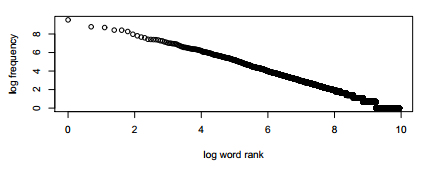
\includegraphics[scale=1]{lestrade} \centering
\caption{The logarithm of word frequency against the logarithm of word rank in \emph{Moby Dick}, taken from Lestrade (2010).}
\end{figure}

Again, we see that a few words are used a lot, while most are used only once or twice.

What holds for individual words must also hold, at least to a certain extent, for combinations of words: some combinations are much more frequent than others. Because these combinations are also more likely to end up in the training material, even with relatively few training material, a context-sensitive system will perform much better than one would expect on the basis of pure chance. On the other hand, once most of the frequent combinations are covered, it takes more and more training material to improve the results just a little bit. This means we also expect a loglinear distribution for the effect of the amount of training material on the results of a word prediction system. \citeA{vandenbosch11} shows this is indeed the case: in his system, the step from 100 to 900 words in the training material, roughly 6\% more keystrokes could saved (from 15\% to 20\% keystrokes saved), whereas the same is true for the step from 1000.000 to 10.000.000 words (from 40\% to 46\%).

A fact both \shortciteA{Lesher+99} and \shortciteA{vandenbosch11} note is that it is not possible to reach 100\% of the keystrokes by simply going on doubling the amount of training material; at a certain point adding more training material does not seem to help anymore. \shortciteA{Lesher+99} hypothize that where that boundary lies depends on how much context the algorithm uses: when more words from the context are used, much more combinations are possible, and thus more training material can be useful. In a hypothetical language with 10 words, 10 contexts are possible when using 1 word as the context, but $10*10*10 = 1000$ contexts are possible when using 3 words as the context. Thus, the larger the context the word prediction system uses, the more contexts are possible, and thus the more the system benefits from having a lot of examples.

As a practical side-note, when using millions of words and all possible combinations between them, and also more context than just two words, a matrix as the one in \ref{matrix} quickly becomes impractical. Modern word predictions systems search through the training material and collect a number of similar contexts. The word that follows most of these contexts will be the word predicted. So when a new context like \emph{You like} is given to such a system, instead of looking it up in a matrix, it compares it to all contexts in the training material. An exact match will be found in the sentence \emph{You like fishing}, and thus \emph{fishing} will be predicted. Because comparing a new context to thousands of contexts in the training material often takes too much time to do real-time predictions, these comparisons can also be done beforehand, which reduces the process to a decision tree \shortcite[among others]{daelemans+97, vandenbosch+08, vandenbosch11}. The system that will be described in this thesis also uses this technique. See chapter \ref{algorithm} for a detailed description of the algorithm.

\subsubsection{Adding linguistic knowledge} \label{linguistic_knowledge}
A basic context-sensitive system, as described in the previous paragraph, knows which words are likely to follow each other, but has no idea of the more 'abstract', higher-level rules that might exist in language. A logical next step might thus be to add explicit linguistic knowledge to the system. For example, we know from (very basic) theoretical linguistics that in Dutch a neuter word like \emph{raam} 'window' cannot follow the common gender article \emph{de} 'the', and that in English adverbials of time always follow adverbials of place. Possibly, this kind of knowledge can help the word prediction system in doing more accurate predictions.

A large part of the authors in the field of word prediction indeed try to include linguistic knowledge in some way. A relatively simple approach is to use Part of Speech tags besides orthographical representations of words, as do \shortciteA{carlberger+97}, \shortciteA{Fazly+03} and \shortciteA{copestake97}. This works similar to the ortographical approach, but this time the system is trained to know what PoS-tags are likely to follow each other (instead of which words). So besides words, the system also predict PoS-tags, and these predicted tags are then used to limit the pool of predicted words. For instance, if the system predicts \emph{work}, \emph{worst}, and \emph{world}, and also expects a noun, \emph{worst} is ruled out because it is an adjective.

A deeper approach is to parse the sentence so far, as done by \shortciteA{Matiasek+02} and \shortciteA{garay-vitoria+97}. This parse can of course only be partial, as the user is still in the process of forming it. The result is then compared to a pool of known syntactic rules for the language. This rule will predict the PoS-tag of the next word, which will again be used to limit the words predicted by another part of the system. \shortciteA{Matiasek+02} go even further and try to take into account compounds, as encountered in languages like Dutch, German and Swedish. If the user uses the backspace to delete the automatically generated space (that is, if the user actively informs the system he/she intended to write a compound here), the compound module is activated. This module tries to predict the rest of the word on the basis of corpus information, like how often all possible continuations of the word are part of a compound, and how often all continuations occur in this context.

Interestingly, most authors conclude that including linguistic knowledge improves the results, but only slightly \shortcite[among others]{garay-vitoria+97, Fazly+03}. As \shortciteA{hunnicutt87} puts it: 'It appears [the implemented grammar] gives small reward for a great deal of effort if one looks at a measure such as keystroke savings'. An explanation for this could be that most of the linguistic knowledge is already covered by the orthographical approach; for our Dutch example, a basic context-sensitive system in practice will only predict common gender nouns after \emph{de}, because those are the only words it has seen at this place in the training material \shortcite{Fazly+03}. That is, because the system has only seen grammatical training material it is very likely to stick to the rules of the language 'by accident'. On top of that, including linguistic knowledge comes with two main downsides: 

\begin{enumerate}
\item The automatical tagging and parsing requires a lot more computing power.
\item It requires tagged and parsed training data. Whereas written material is available for the biggest part of the world's 7000 languages, I estimate tagged and parsed material is available for only 50 of them, which limits the number of languages the system could be used for to less than 1\%.
\end{enumerate}

Because of this, \shortciteA{Fazly+03} even note that adding explicit linguistic knowledge 'might not be considered worth the considerable extra cost that it requires'.

\subsubsection{Adding other knowledge} \label{more_knowledge}

Context-sensitivity, in particular when using a lot of training material, is most powerful when it comes to collocations (for example, \emph{in combination with}, \emph{on the basis of}), i.e. when it comes to language. However, humans use more than knowledge of language alone to predict what somebody is going to say; we also take into account what the speaker typically says, and what the speaker is talking about. For instance, the input \emph{wed} can be very likely to refer to \emph{Wednesday} when making an appointment for next week, whereas it can also be very likely to refer to \emph{wedding} when talking about a marriage. In other words, besides the linguistic context, we also want to give the system some 'real world' context.

One way to give some of this kind of knowledge to word prediction systems is to use training material from the same domain; \shortciteA{verberne+12} show that trying to predict Wikipedia text, tweets, transcriptions of conversational speech and Frequently Asked Questions all worked best when using texts from the same type (i.e. training on Wikipedia text to predict Wikipedia text). Furthermore, they show that questions about neurological issues, for which little training material was available, could best be predicted with the corpus that was closest in terms of topics discussed: the medical pages from Wikipedia. 

\citeA{vandenbosch11} takes a completely different approach and tries to make a word prediction system learn about register and topic on the fly with a \emph{recency buffer}. This buffer stores the $n$ latest words; if a word the user is keying in matches one of the words in the recency buffer, this word is suggested instead of what the system would actually have suggested. The idea behind this is that if the user is writing about, for example, traveling, words like 'go', 'hotel', and 'see'  will always be in the buffer and thus be suggested very quickly. In other words, the systems learns about the user and the topic on the fly.

Although both approaches help to increase the number of keystrokes saved, they also have downsides: for the system by \citeA{verberne+12} training texts in the same genre are needed, which might not be available, whereas the system by \citeA{vandenbosch11} ignores context information that it should weigh more intelligently. For example, while a context-sensitive text-prediction system will probably be able to predict \emph{to} for the sentence \emph{they were going t...}, the one with the recency buffer will predict \emph{they}.


\subsection{Idiolects} \label{idiolects}

\subsubsection{The concept}
Almost every claim done in the field of linguistics concerns language as a whole; whether the subject of investigation is a particular syntactic construction, phonological variable, or some other linguistic phenomenon, the results are always supposed to hold for an entire language variety. The concept of an idiolect, the language of only one person, is well-known, but rarely ever mentioned \cite{mollin09, barlow10, louwerse04}. According to \citeA{mollin09} it is a 'neglected area in corpus linguistics', and \citeA{barlow10} states that the term 'is distinguished by the fact that there is probably no other linguistic term in which there is such a large gap between the familiarity of the concept and lack of empirical data on the phenomenon.' This is remarkable, since 'idiolects are the only kind of language we can collect data on', as \citeA{Haugen72} points out; a language variety essentially is nothing more than a collection of idiolects.

Part of the lack of research in this area can of course be explained by practical limitations (it is hard to collect a lot of data for one person, let alone doing this for multiple persons), but theoretical views have also played a role: for decades, generativism has been the leading linguistic framework. Generativism focuses on \emph{langue} rather than \emph{parole}, and views deviations in actual usage as uninteresting exceptions to an otherwise perfect abstract system. This view was mainly shared by sociolinguists at the time; as \citeA{labov89} puts it: 'language is not a property of the individual, but of the community. Any description of a language must take the speech community as its object if it is to do justice to elegance and regularity of linguistic structure'. However, \citeA{carden70}, himself a generative linguist, points out: 'differences among idiolects have long been an embarrassment for transformational grammarians'.

\subsubsection{Empirical evidence}
Now that usage-based theories of language become increasingly more accepted, and the progress in technology and in particular the internet has facilitated collecting, storing and working with large amounts of data, these objections to studying idiolects slowly vanish. One of the first publications investigating idiolects quantitatively is that of \citeA{mollin09}. She created a corpus of speech by the former Prime Minister of the United Kingdom Tony Blair, and compared this to the British National Corpus. Focussing on maximisers ('absolutely', 'totally') and the adjectives, verbs and adverbs they cooccur with, she has compiled a list of collocations that are used much more by Blair than by the general language community. \citeA{barlow10} investigated speech patterns of five White House Press Secretaries, using transcripts of spoken language available on the internet and dividing them in samples of 200.000 words. He compared the frequencies of bigrams and trigrams (like \emph{of the}, \emph{that we} and \emph{and that's}) and discovered that there are significant differences between individual speakers. Interestingly, however, when frequencies from one sample were compared to frequencies from another sample by the same speaker, they were very consistent. For example, Ari Fleischer rarely uses the bigram \emph{we are} in sample 1, and this is also the case for samples 2, 3 and 4, while the opposite is the true for Scott McClellan. To make sure these differences cannot be attributed to lexical preferences, Barlow repeated his research with POS $n$-grams ([article, noun], [preposition, verb], etc) and grammatical constructions ('\emph{noun} of the \emph{noun}',  'will' vs 'going to', usage of the passive, etc.), and shows similar results.

\subsubsection{Practical use}
The reality of idiolects cannot only be seen through the efforts of corpus linguists, however. \citeA{Coulthard04} gives a number of anecdotes where the notion of idiolects have been helpful in court. The most clear example is the story of the so-called 'Unabomber'. This person sent various hand-made bombs to \textbf{un}iversities and \textbf{a}irports (hence the nickname) from 1978 to 1995, killing 3 persons and injuring 23. In 1995, he offered six major newspapers to stop his attacks if they would publish a manuscript he had written, entitled \emph{Industrial Society and its future}. The Washington Post decided to do so. Three months later, a man contacted the FBI, claiming the language looked very similar to the language of his brother, a mathematician called Ted Kaczynski. He had recognized in particular the phrase 'cool-headed logician' to be part of his brother's idiolect. In the cabin where Kaczynski was living at the moment, indeed a wealth of bomb components were discovered, and FBI researchers determined that other texts that were found there could only have been written by the same person. Kaczynski was sentenced to life in prison with no possibility of parole. 

This example shows the concept of idiolect might be more than just an abstract concept used by linguists. It cannot only only be tested empirically, but is actually something the layman can understand and even recognize. Furthermore, this example shows the concept of idiolect might actually robust enough for practical applications.

\subsection{Using idiolects for word prediction} \label{linking}
As was explained at the end of section \ref{more_knowledge}, both the approach of \citeA{vandenbosch11} and \shortciteA{verberne+12} of adding more knowledge to the word prediction systems have downsides: the system by \citeauthor{vandenbosch11} uses information that easily available, but cannot be used in a context-sensitive way, and the system by \shortciteauthor{verberne+12} is context-sensitive, but uses information which might not be easily available. In this thesis, a word prediction system based around the concept of idiolects will be built: a system that tries to predict what the user is going to write \emph{on the basis of his  or her own language}. The idea behind is that there is a much higher chance that a system will be able to correctly predict what somebody is going to write if it can look at things this same person has produced earlier, instead of things somebody else using the same language has produced earlier. These idiolect data (1) are more likely to be easily available (for example, by using emails, papers, blogposts, tweets or messages by that same author) and (2) can be processed beforehand, and thus can be used in a context-sensitive system. In other words, the best parts of both approaches will be combined.

\subsection{The rest of this thesis} \label{restofthisthesis}
As was explained in detail in section \ref{word_prediction}, word prediction systems work with an algorithm and a language model. Language models are formed out of training material, which simply is a large collection of 'example language' - I used the sentences in \ref{training} to illustrate this. To built an as good as possible word prediction system, it is essential to make both the algorithm and the language model as good as possible, so this is exactly what I will do in the rest of this thesis: chapter \ref{algorithm} is about the algorithm, chapter \ref{model} is about the language model. The thesis will be concluded in chapter \ref{conclusion}. In chapter \ref{algorithm} I will start with a very simple algorithm, and then slowly makes it more complicated. After each addition, little experiments will show to what extent it improves the system. In chapter \ref{model}, various models are compared to each other, to get an idea of which model will work the best for which situation. 





\section{The algorithm: Soothsayer} \label{algorithm}

\subsection{Introduction}

The goal of this chapter is to build the best word prediction algorithm possible, from the ground up. We will start with a very basic application that uses word uniqueness thresholds to predict the word the user is keying in, and add more components and smaller improvements step by step. I have given the resulting system the working title \emph{Soothsayer}, for ease of reference. 

Before I can start, however, there are three things I want to discuss: 

\begin{itemize}
\item Soothsayer's architecture, so the reader has an idea of how all components described below work together.
\item How I evaluate the system, so there is objective information on whether an addition improves the prediction accuracy.
\item What Soothsayer is not, i.e. what is the scope of this project.
\end{itemize}

These topics are topics are discussed in sections \ref{ss_intro}, \ref{evaluation} and \ref{whatnot} respectively.

\subsubsection{Soothsayer's architecture} \label{ss_intro}
Soothsayer works with independent modules. A module can be seen as a function that takes some input (for example, the letters of the word the user is currently keying in) and uses a language model to generate:

\begin{enumerate}
\item The most likely prediction
\item The second most likely prediction
\item The third most likely prediction
\item In case of a context-sensitive module, how many other predictions the model provided
\end{enumerate}

Modules can be either context-insensitive or context-sensitive, as will be explained in much detail in section \ref{ci} and section \ref{cs} respectively, and use one language model. In a set-up with two language models we thus have four possible modules:

\begin{table}[h]
\begin{tabular}{lll} 
Module&Type&Model\\
\hline
1&Context-sensitive&model 1\\
2&Context-insensitive&model 1\\
3&Context-sensitive&model 2\\
4&Context-insensitive&model 2\\
\end{tabular} 
\caption{A possible module set-up for Soothsayer}
\end{table}

Modules can be concatenated in such a way that a second module takes over once the first modules no longer has predictions, a third module takes over once the second one no longer has predictions, etcetera. This makes it possible to use multiple prediction techniques \emph{and} multiple language models in one prediction system.

For clarity, a quick overview of the terms: Soothsayer is a \textbf{word prediction system} which can consist of one or multiple \textbf{modules}. A module in turn consists of a particular \textbf{algorithm} (for example, the context-insensitive one), and a \textbf{language model}. A language model is created on the basis of \textbf{training material}. On several places in this thesis, the reader may get the impression the language model and the training material is the same thing; for example 'a system trained on tweets' can be used interchangably with 'a system using the tweets model'. However, keep in mind the language model is what the system actually uses to make its decisions, whereas the training material is source used to create this language model.

\subsubsection{Evaluating additions} \label{evaluation}
In this chapter, I will propose an addition to Soothsayer and then measure to what extent it improves the number of keystrokes saved several times. But how does one measure how many keystrokes are saved exactly? In other words, what is the best way to evaluate a word prediction system?

In the literature so far, there is still discussion on what is the best way to evaluate word prediction systems. A very straightforward evaluation might be to calculate the percentage of correctly predicted words (the so-called \emph{hit-ratio}), but as \citeA{Garay-Vitoria+06} note, this is not not enough: a system that has 100\% of the words correct, but only gives this prediction at the last letter of every word saves very few keystrokes. A more natural way might be to test with real humans, and measure how much time they save when using the system \shortcite[among others]{carlberger+97,koester+98, Garay-Vitoria+06}. However, this is a costly and time-consuming task, as the participants will need a considerable amount of time to get used to the system. Therefore, I will evaluate Soothsayer by simulating somebody keying in a text, and simply counting how many keystrokes this virtual user does not have to do when using the system. 

However, even when using simulations, there are multiple ways to evaluate the system. One possibility is to provide the user with a list of the $n$ most likely predictions \cite{Lesher+99,Fazly+03}. This approach has the advantage that it results in high percentages of keystrokes saved - in particular when $n$ is set to a high value, because this means the system can do multiple guesses at once, while only one has to be correct. As \citeA{vandenbosch11} notes, however, this also has important downsides: 

\begin{quotation}
[I]n many devices and circumstances it is inefficient or impossible to present [...] suggestion lists. Inspecting a list of suggestions also poses a larger cognitive load than checking a single suggestion, and furthermore it is unclear how scrolling, browsing and selecting items from this list should be counted in terms of keystrokes.
\end{quotation}

For this reason, I will follow \citeA{vandenbosch11} and always calculate the number of keystrokes that could have been saved when the user was presented only one prediction at a time. Predictions can be accepted with the space key. Because this is sometimes problematic (for instance, if the user wanted to type \emph{sun}, but Soothsayer predicts \emph{sunday}, hitting space would lead to the wrong word), a rejection is also calculated as a keystroke. The number of keystrokes that can be saved if the word prediction system works this way will be called \textbf{Classical Keystrokes Saved} (CKS) in the remainder of this thesis.

On the other hand, current popular smartphone applications suggest this approach might be too strict. The popular smartphone application SwiftKey\footnote{\url{http://www.swiftkey.net/}} always shows the user three predictions, which seem to be (1) what the user has keyed in so far, (2) the most likely prediction and (3) the second most likely prediction. In case the user has not yet started typing the next word, option (1) is replaced by the third most likely prediction. Because smartphones use a touchscreen as an input device, no extra keystrokes are needed. The percentage of keystrokes that can be saved when two (and sometimes three) predictions were shown will be referred to as \textbf{SwiftKey Keystrokes Saved} (SKKS).

A thing to notice is that both measures reflect the percentage of keystrokes saved in an ideal situation; that is, when the user accepts a correct prediction immediately once it is available. As will be discussed further in section \ref{early}, this is not necessarily the case. 

\subsubsection{What Soothsayer is not} \label{whatnot}
There are many possible approaches to take when building an word prediction system. Because it would take too much time to try all of these approaches (and all combinations of them), I had to set limitations. Therefore, before I explain and defend the workings of Soothsayer, I would like to list the most important decisions, so the reader has a rough idea of what is coming (and what is not). 

\begin{itemize}
\item \textbf{Soothsayer does not predict more than one word at a time}. Some scholars have investigated the possibility to predict multiple words at the same time \shortcite[among others]{Lesher+99,greenberg+95}. This can very fruitful: if a word prediction system knows that \emph{on the b} should be \emph{on the basis of} it makes more sense to offer this as a whole, instead of first asking whether \emph{basis} is correct. However, multiword prediction comes with a lot of downsides: every extra word that is predicted greatly increases the chance of making an incorrect prediction, it is unclear what a user should do if he/she accepts the first word, but not the second word (or vice versa), and how this should be counted in terms of keystrokes. Furthermore, giving multiple words forces the user to plan ahead a few words while typing, which might not be how the user prefers to write. A useful side effect of predicting only one word at a time is that the space key can be used as an accept button \cite{Garay-Vitoria+06}.

\item \textbf{Soothsayer does not focus on one specific domain of word prediction, but works for word prediction is general}. I expect query completion (i.e. Google completing what you wanted to search for) is the most-used form of word prediction at the moment. It is, however, a relatively small and simple form of it, that probably works with popularity statistics: if your query matches a query a lot of other users also used, this query is suggested. Although this is a smart system that works well, it can only be used for query completion. Soothsayer, on the other hand, can be used for query completion, but also for a lot of other things.

\item \textbf{Soothsayer is not designed for mobile phones, but can be integrated into any kind of software, on any device}. When discussing this subject with others, I noted that word prediction is often confused with T9. T9 is a system in which every number corresponds with 3 or 4 characters (\emph{1} = \emph{.,!}, \emph{2} = \emph{abc}, \emph{3} = \emph{def}, etc.). A T9 system allows the users to press all numbers only once, and tries to figure out which word the writer probably intended; for example, \emph{233} can correspond to \emph{bed}. Although there is some language technology involved in systems like these (the system should know enough about language to figure out \emph{aef}, \emph{cfe} \emph{bde}, etc. are probably not intended), this is not what Soothsayer does; Soothsayer does not try to guess what the user wanted to say \emph{after} the user keyed it in, but \emph{before} he/she did. 

Besides that, Soothsayer is designed to be indepent of device or input method. Instead, it includes a \emph{server mode} and an \emph{HTTP-server mode}, making it very easy to integrate into any piece of software. This means it is very well possible that Soothsayer will be used together with a T9-system one day.

\item \textbf{Soothsayer does not use hand-made, language-specific rules, but is fully language independent}. In the early days of Natural Language Processing, many scholars have tried to build NLP systems by including as much as linguistic knowledge of possible. In terms of a word prediction system, this could for example entail a system that parses the sentence the user has keyed in so far, tries to match this to a pre-made syntactical rule, and predicts something which would be grammatical according to this rule; see chapter \ref{linguistic_knowledge} for more approaches like this.

Soothsayer does not work this way. Instead, it is given as much training material as possible, and tries to learn from that. So Soothsayer might know the noun \emph{kast} probably does not follow the article \emph{het}, but because it has not encountered that during training, not because I told it so exlicitly. As a result of this, Soothsayer is fully language independent: if it is trained on Dutch data, is will predict Dutch words, if it is trained on Swahili, it will predict Swahili words. In fact, the context-sensitive modules will often give correct predictions even when mixing languages - as long as the training material also contained these languages, of course.

\end{itemize}

\subsection{Context-insensitive modules} \label{ci}

Context-insensitive modules only use information of the word the user is currently keying in. In sentence \ref{only_c}, for example, only the c will be used for prediction. 

\begin{examples}
\item I ate too much c \label{only_c}
\end{examples}

This means that a prediction like \emph{communication} is fully possible, despite the context, just because \emph{communication} starts with a c. This also means that at the beginning of a each new word no prediction will be available, because the module has no material to work with.

Despite these limitations, context-insensitive modules can already save a lot of keystrokes, because the first few letters of a word impose enormous limitations on what letters can possibly follow.

\begin{examples}
\item This is good communic \label{communic}
\end{examples}

In sentence \ref{communic}, we already know from \emph{communic} that \emph{ation} or \emph{ative} will follow, simply because these are the only two words that start with \emph{communic}. The first iteration of the context-insensitive module I will propose will be based on this idea: at a certain point in a word, other words are no longer an option. This point is called the \emph{uniqueness threshold}.

\subsubsection{First iteration: using uniqueness thresholds}

The first iteration of the context-insensitive module will take the word the user is currently keying in as the input. If, on the basis of what has been given, only one word is still possible, this word will be returned as a prediction. To know which words are 'possible', the module uses a lexicon. An important characteristic of this approach is that is does not or rarely make mistakes (assuming a large enough lexicon): only words the system is 100\% sure about are predicted.

To test this, I exported all emails I have sent between February 2009 and February 2013, containing 175,168 words. I formed a lexicon on the basis of the first 90\% of the material, and tested on the remaining 10\% - the most recent emails. The testing was done by simulating a user keying in the material letter by letter. Once the correct prediction was available, the remaining letters of that word were skipped. The percentages were calculated by dividing the amount of skipped letters by the total amount of letters.

This resulted in a \textbf{CKS of 5\%} and an \textbf{SKKS of 5\%}. These are relatively low percentages, but that can be explained by the fact that many of the words are too short to reach their uniqueness thresholds. For example, the word \emph{the} will never be predicted because even when the word is finished, alternatives are still possible (\emph{these}, \emph{there}, etc.).

\subsubsection{Second iteration: using word frequencies}
A solution to the fact that short words never reach their uniqueness threshold can be to give the prediction \emph{before} the word has reached its recency threshold. This can lead to situations where the correct word is predicted long before the uniqueness threshold is reached, which increases the number of keystrokes saved. However, this also means many incorrect predictions will be given; we sacrifice the accuracy of the system. To what extent this is a problem is unclear: at the one hand, the user is forced to accept and reject more predictions while typing, which probably increases the cognitive load, at the other hand all the user has to do to reject a prediction is to continue typing; no extra actions are needed. A systematic investigation of the extra cognitive load during typing while using a word prediction system is beyond the scope of this thesis; because no extra actions are needed to reject the prediction it will be assumed the saved keystrokes are worth the extra cognitive load.

If a prediction is given when multiple words are still a possibility, a system that picks the word with the highest chance of occurring will of course have the best results. These chances are reflected by the frequency of the words in the language. Therefore, each time the users keys in a new letter, Soothsayer will go through a frequency list. The first (and thus most frequent and most likely) word that matches with what has been keyed in so far will be given as a prediction.

To test this, the email corpus from the previous section was used. The simulation showed a much higher percentage of keystrokes can be saved this way: a \textbf{CKS of 20 \%} and an \textbf{SKKS of 27 \%}. For this reason, this second iteration of the algorithm is the algorithm that will be used when referring to the 'context-insensitive' module in the remainder of this thesis.

\subsection{Context-sensitive modules} \label{cs}

Context-sensitive modules make use of the words that came before the current word to limit what words are predicted. For sentence \ref{only_c}, repeated here as \ref{only_c_r}, the context would be the words \emph{ate}, \emph{too} and \emph{much}.

\begin{examples}
\item I ate too much c \label{only_c_r}
\end{examples}

Comparing this context to all contexts seen in training material results in a list of words which often occur together with the words from the context. This approach probably returns words like \emph{cookies} or \emph{cake} (because of the word \emph{ate}), while the word \emph{communication} is no longer an option because it probably did not occur in this context in the training material.

\subsubsection{Word prediction as a classification task}

To make use of the context, Soothsayer approaches word prediction as a classification task. Classification means finding a \emph{class} for an \emph{instance} on the basis of its \emph{features}. For instance, you could say a person (instance) is a man (class) because he has a beard, a low voice, short hair and is tall (features). In some cases, classification is simple: when sorting garbage, you use only 1 feature (material) which results in the correct class (paper, glass, plastic, biodegradable, miscellaneous) 100\% of the time, but in most cases it is not; for instance, for a person with a beard you can be pretty sure it is a man, but not all men have beards. And for the other features, there also are women with low voices, women with short hair and women who are tall. In cases like this, it is the combination of features that (in most cases) will result in the correct class.

For word prediction, we use the context as instance, the words in the context as features, and the word which follows this context as class. This means that instead of only two classes (as in the gender example), we have a separate class for every word that could possibly be predicted. Thus, if we want to predict that \emph{cookies} follows the context \emph{ate too much}, we hope that classifying the instance \emph{ate too much} on the basis of its features (the words \emph{ate}, \emph{too} or \emph{much}) will result in the correct class label \emph{cookies}.

\subsubsection{Nearest neighbour classification}

There are many algorithms to do classification automatically. Soothsayer uses the $k$-nearest neighbour classification method. $k$-nearest neighbour classification (henceforth \emph{KNN}) means that the class is determined on the basis of similar cases in a training corpus. How many cases are taken into consideration, $k$, can be determined beforehand. For example, let us set $k$ to 1 and take the following instances as a training corpus:

\begin{examples}
\item one two three (four)
\item one two and (three)
\item one two plus (four)
\end{examples}

The first three words are the instances, the fourth word (between parentheses) is used as the class label. If we then classify a new instance \emph{one two three}, a KNN algorithm will look at these training instances, and decide whether they are similar enough to taken into consideration. What exactly is taken as the definition of 'similar' differs per algorithm; we will follow the IB1-algorithm \cite{aha+91} and simply count how many features overlap. The instance \emph{one two three} is extremely similar: three of the three features match. We then look at the class of this similar example (four), and give this as a result. Simply said, in this case the context-sensitive module will predict \emph{four} because it had exactly the same context in its training corpus, and that context was followed by \emph{four}.

If we set $k$ to 2, both \emph{one two and} and \emph{one two plus} become a possibility as well: they both have two matching features. If we count instances with the same amount of matching features as 1, we now end up with three similar cases. Because most of these cases have \emph{four} as a class label, four will be predicted. Note that \emph{nearest distance classification} would actually be a better name for what we are doing here: we do not use the $k$ nearest neighbours, but \emph{all} nearest neighbours from the $k$ nearest distances \shortcite{daelemans+97}.

Because the many class labels used for word prediction, Soothsayer always uses a $k$ of 1.

\subsubsection{IGTree}

An important thing to notice from the three training instances in the example is that the third feature is the only feature that has relationship with the class label. The first two features are always \emph{one} and \emph{two} respectively, regardless of the class, and thus cannot be used to find out to which class this instance belongs. This is what is used in the in the IB1-IG algorithm, an variation on the IB1 algorithm mentioned previously: because they have a better relation to the class label, some features are given more weight in the decision process.

The idea that some features can be more useful than others can even be used on a much deeper level to solve another problem: the IB1 algorithm generally is too slow to be used in practical applications, like Soothsayer. While the classification in the example above can be done in a split second, this is not the case for word prediction based on a lot of training material: a training corpus of ten thousand words means that a new instance has to be compared to ten thousand training instances for every character the user keys in. This takes too long, even for powerful computers, and is not necessary. This can be best explained with an example. Let us take the following four instances as our training corpus:

\begin{examples}
\item I ate those (cookies)
\item I ate that (cake)
\item I saw those (zebras)
\item I saw that (elephant)
\end{examples}

Whereas the first feature again has no relation with the class, the second one clearly has: as soon as we see \emph{ate}, we know that the classes \emph{zebras} and \emph{elephant} are no longer an option, and that it is of no use to 'keep them in mind' as an option.

This is exactly how the IGTree algorithm \cite{daelemans+97} works: it calculates which features contain most information about the class labels, and orders the features from most informative to least informative. It then goes through these features one by one, and at each point 'throws away' the training instances that are no longer an option. This reduces classification to making a small number of decisions (in our case 3, because we have 3 features), instead of comparing thousands of strings. A possible decision tree for the training instances above can be seen in \ref{igtreetree}.

\qtreeshowframes 

\begin{examples}
\item \Tree [.{\emph{ate} or \emph{saw}?} [.{ate: \emph{those} or \emph{that}?} {those: cookies} {that: cake} ] [.{saw: \emph{those} or \emph{that}?} {those: zebras} {that: elephant} ]] 

\label{igtreetree}
\end{examples}

But what happens if we ask IGTree to classify \emph{I ate these}? At the second node, \emph{these} is not one of the features, so the algorithm cannot make a decision. If a classification gets 'stuck' somewhere, which is almost always the case because the users can of course type anything they want, Soothsayer asks the algorithm to return everything which was still a possibility at that point. In our example, these are the classes \emph{cookies} and \emph{cake} - note that both are indeed possible words, because the classifier still used the feature \emph{ate}. For each possible class, \emph{confidence values} can then be calculated. Confidence values correspond to the percentage of all instances still possible that had that class. The result for \emph{I ate these} in our example would thus be \emph{cookies} with a confidence value of 0.5 (1 of the 2 instances still possible had this class), and \emph{cake} with a confidence value of 0.5 (1 of the 2 instances still possible had this class). If, however, there would have been two more examples with the word \emph{ate} in them that were followed by \emph{cake}, \emph{cake} would have a confidence of 0.75 (3 of the 4 instances still possible had this class), and \emph{cookies} would have a confidence value of 0.25 (1 of the 4 instances still possible had this class).

In practice, what Soothsayer's context-sensitive modules do is:

\begin{enumerate}
\item Starting \emph{Timblserver}, a software suite of Memory-based Learning software, which includes IGTree. Timblserver is similar TiMBL, but get its input using the Transmission Control Protocol. This allows Soothsayer to keep the program running, instead of reloading the tree into memory every single time a classification is needed.
\item Every time the user keys in a character, collecting the last three words, and sending them to the Timblserver.
\item Collecting the output (the classes, thus the word predictions, that Timblserver returned), and picking the word that matches with what already has been keyed in so far. If more words match, Soothsayer picks the one with the highest confidence.
\item Returning this word as a suggestion.
\end{enumerate}

\subsubsection{The experiment}

To investigate how many keystrokes can be saved when using context information, as described in the previous paragraphs, an experiment very similar to the experiment for the context-insensitive modules was carried out: a training corpus was created on the basis of 90\% of all of the emails I sent between February 2009 and February 2013, and the results were tested on the remaining 10\%. The percentages were calculated by dividing the amount of skipped letters by the total amount of letters. This resulted in a \textbf{CKS of 24\%} and an \textbf{SKKS of 27\%}.

\subsection{Other decisions}

\subsubsection{Concatenating context-sensitive and context-insensitive modules} \label{concat}
In the previous two sections, we saw that the context-insensitive module had a CKS of 20\% and an SKKS of 27\%, whereas the context-sensitive one had a CKS of 24\% and an SKKS 27\%. This means that using a context-sensitive module over an context-intensive only gives us an improvement of 4\% for the CKS and no improvement for the SKKS, while it is much more complicated and computationally expensive. Is using context-sensitive modules worth that?

The answer, as I will show, is yes. The context-sensitive module learns about which words in the training texts typically follow eachother, and thus is powerful when it comes to the more frequent, fixed combinations of words and words that often occur in each other's context, but fails when it comes to words that are also frequent, but were not used earlier in this context. The context-insensitive module, on the other hand, can predict any word, as long as it has been used before, but knows nothing about fixed combinations. In other words, one module succeeds where the other fails, and vice versa; there is very little overlap in the situations in which they both do the correct prediction. 

This means that it would make sense to concenate context-sensitive and context-insensitive modules, but in which order? Should the context-insensitive module take over when the context-insensitive module no longer has suggestions, or the other way around? Based on the fact that the context-sensitive module alone performs a bit better, it is likely that the results will be slightly better when the context-sensitive module is tried first. Two simulations confirmed this, as shown in table \ref{results_concat}.

\begin{table}[h]
\begin{tabular}{l|ll} 
&CKS&SKKS\\
\hline
Context-insensitive$\rightarrow$context-sensitive&30&35\\
Context-sensitive$\rightarrow$context-insensitive&33&37\\
\end{tabular} 
\caption{Percentage of keystrokes Soothsayer saves with a context-sensitive module first and a context-insensitive module first} \label{results_concat}
\end{table}

For this reason context-sensitive modules will always be ranked before context-insensitive ones in the remainder of this thesis.

\subsubsection{Attenuation}

In the experiments presented so far speed has not really been an issue, because the training corpus was relatively small (175,186 words). However, in section \ref{simple_exp} a background corpus that is considerably larger (55,212,868 words) will be used. As the experiments below will show, this results in IGTrees too large and thus too slow for realtime use.

To solve this problem, I will use a (simplified version of a) solution from the field of syntactical parsing called \emph{attenuation} \cite{eisner96}. This entails that all words in the training material that occur less often than a particular threshold, and thus are extremely rare and unlikely in all but one of the training contexts (thus, unlikely in more than 99.99\% of the cases) are replaced by a dummy value. In section \ref{context-sensitivity} we saw that Zipf predicts that the group of words that only occurs once is actually the biggest group, so merging them all into one word will make the IGTree considerably smaller and thus faster. So to summarize, attenuation speeds up the classification, and removes useless cases. For Soothsayer, the attenuation value of 3 was chosen after some trial-and-error; other values give very similar results.

For the training corpus used in this chapter, the effects of attenuation are summarized in table \ref{results_att}.

\begin{table}[h]
\begin{tabular}{l|lll} 

&CKS&SKKS&Duration in seconds\\
\hline
Without attenuation&33&37&752\\
With attenuation&33&38&660\\
\end{tabular} 
\caption{Percentage of keystrokes saved and simulation times with and without attenuation.} \label{results_att}
\end{table}

The table shows the duration of the simulation decreased when the attenuation was turned on. As noted before, however, for this relatively small training corpus this was not needed: with a test text of 105922 characters, the 752 seconds Soothsayer takes for the simulation without attenuation already mean an average 141 of keystrokes per second could be achieved. This is well above the 8 keystrokes per second for fast typists, according to \citeA{kieras+94}.

For the larger background corpus used later in thesis, we do see important differences, however. [[exp still need to be done, currently waiting for an empty pony]]

%Grote corpus

\subsubsection{Handling morphology} \label{early}
In section \ref{linguistic_knowledge}, we saw that the small improvements that could be made by adding explicit linguistic knowledge were not worth the effort. However, adding linguistic knowledge is not the only way to work with morphology. In this section, an approach that focusses on form rather than content is suggested.

The biggest problem with morphology is that it changes word forms. This is problematic for word completion, in particular with compounds and suffixes. For example, imagine a user has already written sentence \ref{morphology}, and wants to write the word \emph{cookies}:

\begin{examples}
\item I would really like the c \label{morphology}
\end{examples}

If in the training material the word \emph{cookie} was much more frequent, Soothsayer will suggest that instead of \emph{cookies} - in this case incorrectly. Normally, when a prediction is wrong, the algorithm will find out because the user keys in another letter (so the predicted word no longer matches what the user is typing), but that technique will not work here. For words that only differ in their suffix, the point of difference is at the end of the word, when there is nothing left to predict. Even if the correct word is the second most likely prediction, this will not be suggested, because Soothsayer has no reason to switch prediction.

However, there is a clue Soothsayer could use: normally, when a prediction is right, the user will accept it, instead of going on writing. He/she might not accept it immediately (typing often goes faster than mentally processing predictions), but once the user has not accepted a prediction for more than three keystrokes in a row, it gets more and more likely the user keeps typing because the prediction is wrong. In that case, the second most likely prediction could be displayed, which in many cases will be the word with the second most likely suffix.

This approach, which I will call \emph{early prediction switching}, is in many ways similar to the use of frequency lists instead of uniqueness thresholds for the context-insensitive module. The original system only switched prediction when it was completely sure the original prediction was wrong, just like the context-insensitive module originally only showed a prediction when it was completely sure. The system with early prediction switching needs less input, and already switches when it is likely (but not certain!) switching is necessary, just like the context-insensitive module with the frequency lists, which already gives a suggestion when it has something which is likely, but far from certain.

The results are displayed in table \ref{results_epd}. As can be seen, when the results are switched almost immediately if the user does not accept (after 1 or 2 keys), the there is slight improvement of the CKS, but this improvement disappears again once the system is set to be more cautious. From my own experience with the system (both hands-on and watching other people play with it), I know that typing 2 to 3 keys before accepting the prediction is quite normal. Therefore, early prediction switching will be turned off in the remainder of this thesis.

\begin{table}[h]
\begin{tabular}{l|lll} 

&CKS&SKKS\\
\hline
Without early prediction switching&33&37\\
Early prediction switching after 1 key&35&39\\
Early prediction switching after 2 keys&35&39\\
Early prediction switching after 3 keys&33&37\\
\end{tabular} 
\caption{Percentage of keystrokes saved with and without early prediction switching.} \label{results_epd}
\end{table}

\subsubsection{Recency} \label{rb}

Although in chapter \ref{intro} idiolects are presented as a context-sensitive alternative to the recency buffer by \citeA{vandenbosch11}, the recency buffer can also be used as an addition to idiolects. As \citeA{church02} shows, the probability that a words occurs twice in a short stretch of text is far higher than its  frequency in language would suggests, which is mainly related to the topic - for example, in this text the words \emph{prediction}, \emph{keystrokes} and \emph{context-sensitive}  occur far more than one would expect on the basis of their frequency, because these terms are related to the topic of this text. 

Whereas knowledge about topics is also partly covered by the idiolect model (it knows what kind of topics the user likes to talk about), the recency buffer by definition uses more recent text (that is, material from the same text), and might this way be able to do more accurate predictions. For example, if the user is writing about a new woman he/she has met and mentions here name several time, the idiolect model will fail to predict that name every time (unless, of course, the name already occurs in the training material), while the recency buffer will get it after only one mention.

To test this, a recency buffer has been built into Soothsayer as a module. Like a regular module, the recency buffer takes over when the previous module has no suggestions. However, unlike a regular module, the recency buffer does not use a pre-made language model, but needs to be updated every time a new word is completed. The buffer remembers the $n$ most recent words, and suggests the most recent one that matches with the word that is currently being keyed in. Following \citeA{vandenbosch11}, $n$ was set to 300. If no word matches, the next module will take over. The results of adding a recency buffer to various places in the current chain are displayed in table \ref{results_rb}.

\begin{table}[h]
\begin{tabular}{l|lll} 

&CKS&SKKS\\
\hline
Without recency buffer&33&37\\
\textbf{Recency buffer}$\rightarrow$context-sensitive module$\rightarrow$context-insensitive module&32&37\\
Context-sensitive module$\rightarrow$\textbf{recency buffer}$\rightarrow$context-insensitive module&34&39\\
Context-sensitive module$\rightarrow$context-insensitive module$\rightarrow$\textbf{recency buffer}&34&39\\
\end{tabular} 
\caption{Percentage of keystrokes saved with and without a recency buffer.} \label{results_rb}
\end{table}

As can be seen, adding a recency buffer only results in slight improvements. As will be investigated in detail in sections \ref{recbuf} and \ref{twitter_idiolects}, this is related to the nature of the training material: the material used for the experiments in this chapter are idiolect data, which has roughly the same kind of 'information' about the language of the user as the recency buffer. In sections \ref{recbuf} and \ref{twitter_idiolects}, the recency buffer will added to various models to see how much it improves. For now, the important thing is that it indeed improves the results. 

Another thing to notice is that the buffer should not be added to the beginning of the chain, as that will block the more intelligent context-sensitive module. As was noted in section \ref{word_prediction}, while the context-sensitive module will probably be able to predict \emph{to} for the sentence \emph{they were going t...}, the one with the recency buffer will predict \emph{they}.

\subsection{Overview}
In this chapter, I started with 1 simple context-insensitive module based on uniqueness thresholds, and added improvements step by step. The results of these additions are summarized in the graph below:

\begin{figure}[H] \centering
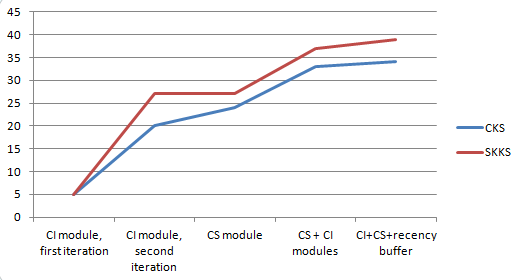
\includegraphics[scale=1]{overview}
\caption{Overview of the improvements made to the algorithm in this chapter.}
\label{overview}
\end{figure} 






\section{The model: idiolects} \label{model}

In chapter \ref{intro}, we saw that both \shortciteA{verberne+12} and \citeA{vandenbosch11} try to give their system information about the style and the content of what they are trying to predict: whereas \citeA{verberne+12} used training material similar to the test material, \citeA{vandenbosch11} made his system learn about the user on the fly. In section \ref{restofthisthesis}, a new approach was suggested: linking the field of word prediction to the field of idiolects. This approach has the advantage that it (1) users material that is usually easily available \emph{and} (2) can use context-sensitivity. Now we have a working algorithm, as described in chapter \ref{algorithm}, we can test this suggestion empirically by comparing the number of keystrokes that can be saved when using various models. The power of idiolects will be shown with a simple experiment in section \ref{simple_exp}. In section \ref{background}, we will see that general models can still be useful, however; they can function as a safety-net in case the author use a word or combination of words that very common to the language, but he/she has never used before. Section \ref{recbuf} will show what effect the recency buffer has on these language models.

In section \ref{twitter_idiolects}, these experiment will then be replicated on a much larger scale, using 100 Twitter feeds as idiolects. After that, section \ref{input_networks} will show that the idiolect model can be extended to what will be called a sociolect model: the language of the people the user often communicates with.

\subsection{A simple experiment: idiolects over general models} \label{simple_exp}

\subsubsection{Research question}
As decribed in \ref{restofthisthesis}, I expect that using idiolects, texts written by the user of the word completion system, as training models will save more keystrokes than a general language model. The research question for this first experiment thus is:

\begin{examples}

\item Does using a general language model or an idiolect model lead to more keystrokes saved?

\end{examples}

\subsubsection{Data} \label{data_simple}
This experiment will compare two language models: a model based on the texts by one person, and a general language model. The idiolect consists of all emails I have sent between February 2009 and February 2013, containing 175,186 words. The first 90\% of the material was used for training, the remaining 10\% - the most recent emails - for testing. This is also the language model which has been used for testing in chapter \ref{algorithm}. 

As a control model, a general language model for Dutch will be used. For this, a random selection of blogs, emails and Wikipedia articles from the SoNaR corpus for written Dutch \shortcite{oostdijk+13} was made. These texts were chosen because they were believed to be neither very formal nor very informal. The control corpus consisted of 55,212,868 words.

\subsubsection{Methodology}
To the language models, Soothsayer, the algorithm described in chapter \ref{algorithm}, will be used. Similar to the experiments there, a user keying a text will be simulated. If Soothsayer correctly guesses the next word, or the rest of the current word, it is assumed this virtual user will accept it, and goes on keying in the next word. It is then calculated what percentage of keystrokes was saved when only one suggestion was shown to the user (\textbf{C}lassical \textbf{K}eystrokes \textbf{S}aved), and when two and sometimes three suggestions are shown (\textbf{S}wift\textbf{K}ey \textbf{K}eystrokes \textbf{S}aved). Unlike the experiments in chapter \ref{algorithm}, however, these experiments will not compare two versions of the algorithm, but two language models. Thus, whereas the experiments in chapter \ref{algorithm} kept the model constant, and varied the algorithm (a version with feature $x$ turned on and a version with feature $x$ turned off, for instance), the experiments in this chapter will do the opposite and vary the model while keeping the algorithm constant. 

The module set-ups for the two simulations are shown in table \ref{idiolect_setup} and \ref{generalmodel_setup}. Each row in the table represents a module.

\begin{table}[H]
\begin{tabular}{lll} 
Position&Type&Model\\
\hline
1&Context-sensitive&idiolect\\
2&Context-insensitive&idiolect\\
\end{tabular} 
\caption{Module order for a simple idiolect simulation.} \label{idiolect_setup}  
\end{table}

\begin{table}[H]
\begin{tabular}{lll} 
Position&Type&Model\\
\hline
1&Context-sensitive&general\\
2&Context-insensitive&general\\
\end{tabular} 
\caption{Module order for a simulation for the general model.} \label{generalmodel_setup} 
\end{table}


\subsubsection{Results}

\begin{table}[H]
\begin{tabular}{ll|ll} 
Training material&Test material&CKS&SKKS\\
\hline
General &Text by WS&22&25\\
Idiolect&Text by WS&35&39\\
\end{tabular} 
\caption{Percentage of keystrokes that can be saved when using the general and the idiolect model} \label{results_simple}
\end{table}

Table \ref{results_simple} shows that  using the idiolect model indeed leads to more keystrokes saved. 

\subsubsection{Conclusion}
Despite the fact that the general model contained more than 300 times more words than the idiolect model, much more keystrokes could be saved using the idiolect model. This is consistent with both \citeA{vandenbosch11}, who shows that learning about the author improves the results, and \shortciteA{verberne+12}, who show that using training material from the same genre improves the results.

\subsubsection{Discussion}
As was explained in section \ref{word_prediction}, the accuracy of word prediction really depends on how much training material was used to create the language model. This means that the above results only hold for exactly this amount of training material; by adding more material, the results are likely to improve, by removing material, the results are likely to deteriorate. That must also mean that for idiolect models based on very little training data, the findings of this experiment do not hold. To answer the question how much idiolect data is necessary to be a better choice than the general language model, at least for the current idiolect, I followed \citeA{vandenbosch11} and repeated the above experiments several times, with part of the training data removed. The result are summarized in the learning curve shown in figure \ref{lcurve}.

\begin{figure}[H] \centering
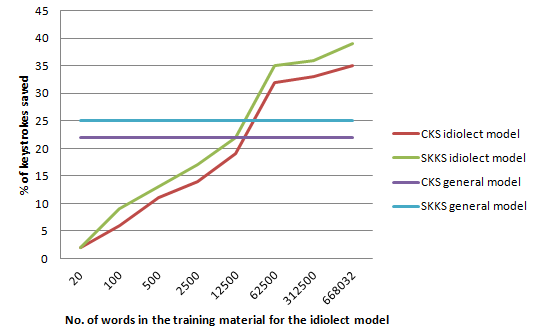
\includegraphics[scale=1]{lcurve}
\caption{The CKS and SKKS of the idiolect model with various amounts of training material.}
\label{lcurve}
\end{figure} 

We see that, as \citeA{vandenbosch11} suggested, to keep improving the results at the same rate, the amount of training material needs to grow exponentially. The example here starts with 20 words, and this number is multiplied by 5 for each step. Furthermore, we see that using the idiolect model starts giving better results  than the general language model somewhere between 12.500 and 62.500 words; roughly when it approaches 0.1\% of the amount of words in the general language model (55,212,868).

\subsection{The general language model as a background model} \label{background}

\subsubsection{Research question}

A next step might be to combine both models. Given their nature, this is very likely to lead to better results: whereas the idiolect model has information on what words, word combinations and constructions a person likes to use, the general model has information on what words, word combinations and constructions are possible in the language. While the idiolect model will do most of the work, the general model takes over once the user starts using language which he/she have never used before, but which is possible in the language. 

Or to phrase it from a more theoretical perspective: although a language variety is nothing more than a collection of idiolects, as stated in chapter \ref{intro}, a language variety can only be called a language variety when the idiolects are very similar; otherwise the language users would not be able to communicate. This should mean that idiolects of other people using the same language variety, although less good than the idiolect, can still contain valuable information.

The research question for this experiment thus is:

\begin{examples}

\item Does using the general language model as a background model for the idiolect model lead to more keystrokes saved than using one idiolect model alone?

\end{examples}

\subsubsection{Data}
As dataset, the corpora described in \ref{data_simple} will be used. However, this time  both corpora will be used in one experiment.

\subsubsection{Methodology}
Again, the algorithm described in chapter \ref{algorithm}, Soothsayer, will be used. As was explained in section \ref{ss_intro}, Soothsayer consists of several modules that function as each other's safety net; if one module fails to deliver a prediction, the next one takes over. This way more than one language model can be easily be used in one experiment.

In which order should the modules be placed? To limit the amount of possible module orders, I will do two assumptions:

\begin{enumerate}

\item The idiolect model should be used before the general model. Since using the idiolect model leads to better results, as shown in section \ref{simple_exp}, it makes sense to try that one first.
\item The context-sensitive model should be used before the context-insensitive model. As shown in section \ref{concat}, the algorithm performs better when context-sensitive modules are placed before context-insensitive ones.

\end{enumerate}

It is not possible to take into account both assumptions: if we want all modules using the idiolect model to go before all modules using the general model, a context-insensitive module has to go before a context-sensitive one. However, if we allow slight violations of one of the two assumptions, we get two possible orders. They are displayed in table \ref{order1} and \ref{order2}. 

\begin{table}[H]
\begin{tabular}{lll} 
Position&Type&Model\\
\hline
1&Context-sensitive&idiolect\\
2&Context-sensitive&general\\
3&Context-insensitive&idiolect\\
4&Context-insensitive&general\\
\end{tabular} 
\caption{Module order with the general model as background model, version 1} \label{order1}
\end{table}

\begin{table}[H]
\begin{tabular}{lll} 
Position&Type&Model\\
\hline
1&Context-sensitive&idiolect\\
2&Context-insensitive&idiolect\\
3&Context-sensitive&general\\
4&Context-insensitive&general\\
\end{tabular} 
\caption{Module order with the general model as backgroun model, version 2} \label{order2}
\end{table}

\subsubsection{Results}

The results are shown in table \ref{results_background}. The first row repeats the results displayed in table \ref{results_simple}, from the previous experiment, the second and third are the results of this experiment. The table shows that using the general model as a background corpus indeed increases the number of keystrokes saved, and that there is no measurable difference between order 1 and 2.

\begin{table}[H]
\begin{tabular}{ll|ll} 
Training material&Test material&CKS&SKKS\\
\hline
Idiolect&Text by WS&35&39\\
Idiolect + general, order 1&Text by WS&39&42\\
Idiolect + general, order 2&Text by WS&39&42\\
\end{tabular} 
\caption{Percentage of keystrokes that can be saved when using the general model as background model} \label{results_background}
\end{table}

\subsubsection{Conclusion}
We saw that using the general language model as a background model indeed increases the number of keystrokes saved. This is because the idiolect model, although it has more knowledge on what is likely to follow, is dependent on what the user has said before, and becomes useless when the user deviates from his/her normal patterns. As long as the user remains within the bounds of the language, the general model can fill this knowledge gap to a certain extent.

Because there was no measurable difference between order 1 and order 2, the choice for one over the other becomes arbitrary. For subsequent experiments with a background model, I will consistently pick order 1.

\subsubsection{Discussion} \label{simple_exp_disc}
Is having a general language model as background model equally efficient for all idiolects? In this section, as a side-track, I'd like to argue this is not the case; it is very likely it depends on how large the gap is the general model can fill. In the main experiment, we saw an increase in the number of keystrokes saved, from 34 \% CKS to 40\% CKS (6\%). To show the benefits are even higher for idiolect models with less good results, I will repeat this experiment with another idiolect: one year of weblogs written by Dutch physician and astronaut Andr\'e Kuipers, from July 2011 to July 2012. This period covers the preparations for Kuipers' second spaceflight PromISSe on Expedition 30 and Expedition 31 (from July to December 2011), the actual space mission (December 2011 to June 2012), and his return to earth (July 2012). The corpus consists of 31,790 words. 

Like in the main experiment, it was calculated how many keystrokes could be saved when using the idiolect model alone, and the idiolect model with a general language model as background model. The results are summarized in table \ref{results_kuipers}. 

\begin{table}[H]
\begin{tabular}{ll|ll} 
Training material&Test material&CKS&SKKS\\
\hline
Idiolect&Text by AK&26&29\\
Idiolect + general&Text by AK&37&40\\
\end{tabular} 
\caption{Percentage of keystrokes that can be saved when using the idiolect of Andr\'e Kuipers, with and without background model} \label{results_kuipers}
\end{table}

These results show again that the algorithm performs much better when it uses the background model. Interestingly, whereas this idiolect alone leads to lower percentages than the idiolect of the main experiment, when using a background model the results are similar. We thus see a much larger increase: 11\% (compared to the 6\% of the main experiment). Apparently, because for the idiolect model of Andr\'e Kuipers less material was available, there is a larger knowledge gap the general language model can fill.


\subsection{The effect of the recency buffer} \label{recbuf}

\subsubsection{Research question}

For the experiments so far, the recency buffer was not used. As suggested in section \ref{rb}, this might be a missed chance: the recency buffer by definition uses more recent input by the user than any other model, and might this way be able to do more accurate predictions. When added to a module using an idiolect model, the recency buffer is expected to have slight improvements, because of the recency. When added to a module using a general language model, however, the recency buffer is expected to have much larger improvements, because here the buffer can also add information about the idiolect of the user. The research question for this simulation thus is:

\begin{examples}
\item To what extent does adding the recency buffer improve the number of keystrokes saved for the idiolect model, the general language model, and a combination of them?
\end{examples}

\subsubsection{Data}

Both the idiolect and the general language corpus described in section \ref{data_simple} will be reused. 

\subsubsection{Methodology}
The experiments described in sections \ref{simple_exp} and \ref{background} will be repeated, but this time with a recency buffer in the module chain. As was discovered in section \ref{rb}, the system loses important information when it is put behind context-sensitive modules, so the recency buffer is always included directly after the last context-sensitive module. This leads to the following context-sensitive module orders:

\begin{table}[H]
\begin{tabular}{lll} 
Position&Type&Model\\
\hline
1&Context-sensitive&idiolect\\
2&Recency buffer&recent words\\
3&Context-insensitive&idiolect\\
\end{tabular} 
\caption{The module order for simulation 1, with the idiolect model and the recency buffer} 
\end{table}

\begin{table}[H]
\begin{tabular}{lll} 
Position&Type&Model\\
\hline
1&Context-sensitive&general\\
2&Recency buffer&recent words\\
3&Context-insensitive&general\\
\end{tabular} 
\caption{The module order for simulation 2, with the general model and the recency buffer} 
\end{table}

\begin{table}[H]
\begin{tabular}{lll} 
Position&Type&Model\\
\hline
1&Context-sensitive&idiolect\\
2&Context-sensitive&general\\
3&Recency buffer&recent words\\
4&Context-insensitive&idiolect\\
5&Context-insensitive&general\\
\end{tabular} 
\caption{The module order for simulation 3, with the idiolect model, the general model and the recency buffer} \label{sim3}
\end{table}


\subsubsection{Results} 

\begin{table}[H] 
\centering
\begin{tabular}{ll|llll} 
Training material&Test material&\multicolumn{2}{l}{Without recency buffer}&\multicolumn{2}{l}{With recency buffer}\\
\hline
&&CKS&SKKS&CKS&SKKS\\
General&Text by WS&22&25&24&27\\
Idiolect&Text by WS&35&39&34&39\\
General + idiolect&Text by WS&39&42&40&43\\
\end{tabular} 
\caption{Percentage of keystrokes that can be saved with and without the recency buffer} \label{recbuf_results}
\end{table}

Table \ref{recbuf_results} shows that, as expected, the recency buffer has the most effect when added to the general language model. Furthermore, we see that, even if there are improvements, they are minimal.

\subsubsection{Conclusion}
In section \ref{rb}, we saw that using the recency buffer only results in slight improvements. That result has been replicated here. The improvement is a little bigger for the general language model, as expected, because here the recency buffer can add some simple idiolect information, besides information about recent language.

\subsection{Using Twitter feeds as idiolects} \label{twitter_idiolects}

\subsubsection{Research question}
Although previous experiments had clear results, these are the results of only one idiolect. It is possible that this idiolect is not representative of idiolects in general; some people might have a much more consistent style of writing than others. It is for a reason that the study of idiolects is sometimes also called the study of \emph{individual differences} \cite{barlow10}. The research question for this section therefore is:

\begin{examples}
\item To what extent do the previous findings hold for other language users?
\end{examples}

\subsubsection{Data} \label{data_twitter_idiolects}
In this experiment, the power of idiolects will be investigated on a much larger scale by using 100 idiolects at the same time. For this, micro-blogging service Twitter will be used, as it essentially is a large collection of idiolects. Twitter\footnote{\url{http://www.twitter.com}} is a micro-blogging service where each Twitter user can submit status updates known as tweets, which consist 140 characters or less. These tweets typically consist of personal information about the users themselves, news or links to other pages on the internet. Tweets are displayed on the user's profile page. 

Using the Twitter API, all tweets of a manually created seed set of Dutch Twitter users were retrieved from January until June 2013. Retweets, language these authors did not produce themselves, were excluded. These seed users were the starting point of an iterative expansion of the set of crawled Twitter uses by following mentions of other users (indicated with the syntax \emph{'@username'}). The goal of this expansion was to find as much active Twitter users as possible for the system to follow, and to capture the network of these users (which we will need for later experiments). The set was extended with 2 users every 30 minutes:

\begin{itemize}
\item One user was selected on the basis of the number of tweets the system had already saved referred to them. Thus to find this person, the system made a frequency list of all \emph{@addressee} mentions. The Twitter user that was highest on this list, but was not already being followed, was added. This way, I could be sure the new person communicated a lot with at least one of the persons the system was already following.
\item Another user was selected on the basis of the number of users the system was already following referred to them. Thus to find this person, the system made a frequency list of all \emph{@addressee} mentions, counting multiple references by one person only once. The Twitter user that was highest on this list, but was not already being followed, was added. This way, I could be sure the new person had a lot of connections to the people the system was already following.
\end{itemize}

The system limited itself to Dutch tweets using a conservative Dutch word frequency list. Addressees receiving non-Dutch tweets were not followed.

Concerning the relation between number of tweets and Twitter users, many scholars have noticed that it follows a Pareto-distribution \shortcite[among others]{asur+10,rui+12}. That is, a very small part of the Twitter users produce a very large part of the tweets\footnote{Another Pareto-distribution is the Zipf-curve discussed in chapter \ref{intro}.}. \shortciteA{heil+09} show that the top 10\% of prolific Twitter users were responsible for more than 90\% of the tweets. \shortciteA{asur+10} suggests this behavior can be found across various social media; for example, according to them 'the top 15\% of the most prolific editors account for 90\% of Wikipedia's edits'. The Twitter data collected for this research show a similar pattern:

\begin{figure}[H] \centering
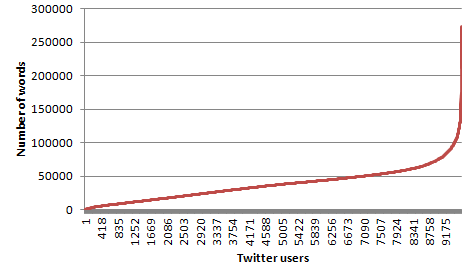
\includegraphics[scale=1]{zipf_twitter}
\caption{The amount of words by all Twitter users followed by the system.}
\label{lcurve}
\end{figure} 

The relatively stable growth in the left part of the graph can be explained by the collection method used, which required the Twitter users to be at least a little active. 

This distribution means that using all or a random selection of Twitter users is not likely to lead to good results, because for most users not much material is available. Therefore, only data from the 100 Twitter users for which there was the most material will be used to build the idiolect models. Twitter accounts run by something other than an individual person (like a company) were excluded manually. The number of words ranged from 61,098 words for the least active user (of the 100 users included in the experiments) to 167,685 words for the most active user. For the general Dutch corpus, the corpus described in section \ref{data_simple} will be used, which had 55,212,868 words.

\subsubsection{Methodology}

The experiments described in sections \ref{simple_exp}, \ref{background} and \ref{recbuf} will be replicated, with the same module set-ups. However, instead of only once, all experiments will now be done 100 times, with 100 different idiolect models. An overview of the experiments and their module set-ups:


\begin{table}[H] \footnotesize
\begin{tabular}{l|l|p{1.2cm}p{1.2cm}p{1.2cm}p{1.2cm}p{1.2cm}} 
Simulation&Experiment&Idiolect, context-sensitive&General, context-sensitive&Recency buffer&Idiolect, context-insensitive&General, context-insensitive\\
\hline
1&1&x&&&x&\\
2&1&&x&&&x\\

3&2&x&x&&x&x\\

4&3&x&&x&x&\\
5&3&&x&x&&x\\
6&3&x&x&x&x&x\\

\end{tabular} 
\caption{Overview of all module set-ups} 
\end{table}

Experiment 1 investigates whether idiolect models or the general language model are more powerful, experiment 2 investigates the effects of using the general language model as background model, and experiment 3 investigates the effect of adding the recency buffer to the idiolect model, the general language model, and both.

\subsubsection{Results}

The results of the simulations are summarized in tables \ref{twitter_results_cks} and \ref{twitter_results_skks}. Because of the number of factors involved, CKS and SKKS are shown in two separate tables for clarity. Both tables show exactly the same pattern.

\begin{table}[H] 
\centering
\begin{tabular}{ll|llll} 
Training material&Test material&\multicolumn{2}{l}{Without recency buffer}&\multicolumn{2}{l}{With recency buffer}\\
\hline
&&Mean&St. dev.&Mean&St. dev.\\
General&Twitter feed&14&5&23&5\\
Idiolect&Twitter feed&23&8&27&8\\
General + idiolect&Twitter feed&26&6&30&6\\
\end{tabular} 
\caption{Mean percentage of keystrokes saved (\textbf{CKS}) and standard deviations for all module set-ups.} \label{twitter_results_cks}
\end{table}

\begin{table}[H] 
\centering
\begin{tabular}{ll|llll} 
Training material&Test material&\multicolumn{2}{l}{Without recency buffer}&\multicolumn{2}{l}{With recency buffer}\\
\hline
&&Mean&St. dev.&Mean&St. dev.\\
General&Twitter feed&16&6&26&5\\
Idiolect&Twitter feed&25&8&28&7\\
General + idiolect&Twitter feed&28&6&32&6\\
\end{tabular} 
\caption{Mean percentage of keystrokes saved (\textbf{SKKS}) and standard deviations for all module set-ups.} \label{twitter_results_skks}
\end{table}

First of all, we see that all main findings could be replicated: 

\begin{enumerate}
\item Using the idiolect model leads to more keystrokes saved than using the general model.
\item Using the general language model as a background model leads to more keystrokes saved than using the idiolect model alone.
\item Using the recency buffer leads to more keystrokes saved.
\item The effect of the recency buffer is the clearest when it is used in addition to the general model.
\end{enumerate}

An ANOVA for repeated measures showed that there indeed was a significant effect of the training material $F(2,198) = 109.495, p > .001$ and whether the recency buffer was used $F(1,99) = 469.648, p > .001$. Contrast analyses revealed that both the differences between the results of the general model and the idiolect model $F(1,99) = 41.902, p > .001$ and the idiolect model and the idiolect model with the background model $F(1,99) = 232.140, p > .001$ were significant.

Interestingly, there also is one difference with previous results. In section \ref{recbuf}, using the recency buffer only resulted in slight improvements; often only 1\%. However, here we see increases around 4\%, and even 10\% for the general language model. This is very likely to be related to another characteristic of the data: as already indicated by the relatively high standard deviations, there is a lot of variation. The results of 4 individual twitter users are shown in table \ref{twitter_users_rb} to illustrate this. These are the results for the module set-up with both the idiolect model and the general language model.

\begin{table}[H] 
\centering
\begin{tabular}{l|llll} 
Twitter user&\multicolumn{2}{l}{Without recency buffer}&\multicolumn{2}{l}{With recency buffer}\\
\hline
&CKS&SKKS&CKS&SKKS\\
2&22&24&30&32\\
93&21&24&29&32\\
34&35&37&35&38\\
43&35&37&36&38\\
\end{tabular} 
\caption{Percentage of keystrokes saved for 4 individual Twitter users, with and without the recency buffer} \label{twitter_users_rb}
\end{table}

Here, we see that for user 2 and 93 adding the recency buffer results in an considerable increase in the number of keystrokes saved, whereas the effect can barely be measured for user 34 and 43. Similar discrepancies can be found for the other research results, as displayed in table \ref{twitter_users}. These are the results without recency buffer.

\begin{table}[H] 
\centering
\begin{tabular}{l|llllll} 
Twitter user&\multicolumn{2}{l}{General model}&\multicolumn{2}{l}{Idiolect model}&\multicolumn{2}{l}{Both}\\
\hline
&CKS&SKKS&CKS&SKKS&CKS&SKKS\\
97&2&3&51&52&50&50\\
90&15&17&12&13&19&21\\
55&23&26&24&26&32&36\\
78&11&13&35&38&35&38\\
\end{tabular} 
\caption{Percentage of keystrokes saved for 4 individual Twitter users, for the idiolect and the general model} \label{twitter_users}
\end{table}

For user 97, we see that the general model alone leads to very few correct predictions, while the opposite is true for the idiolect model. Using the general language model as background model even leads to a decrease in the number of keystrokes saved. We see the reverse situation with user 90, for whom the general model actually did better predictions than the idiolect model. For user 55, we see that using the general language model as a background model leads to a considerable increase in percentage of keystrokes saved, while there is no measurable difference for user 78.

The large individual differences are illustrated in figure \ref{chaos}, where the users were ordered from least to most material. Contrary to expectations before this graph could be produced, no correlation between amount of training material and the results could be detected (Pearson's correlation, $p = .763$); apparently, the individual factor is that much stronger.

\begin{figure}[H] \centering
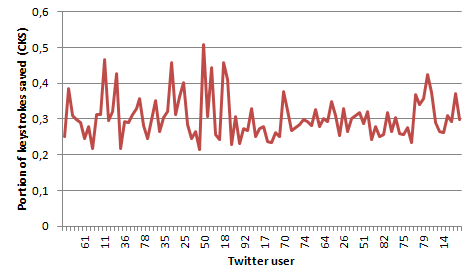
\includegraphics[scale=1]{twitter_chaos}
\caption{The proportion of keystrokes saved for individual Twitter users, when using the best-performing module set-up}
\label{chaos}
\end{figure} 

These differences means Soothsayer performs much better for one than for the other. Using the best-performing module set-up in general, the set-up with the idiolect model, backed up by the general language model, \emph{and} the recency buffer, the worst result is \textbf{22\% CKS} and \textbf{24\% SKKS} for user 90, and the best result is \textbf{51\% CKS} and \textbf{52\% SKKS} for user 97.

\subsubsection{Conclusion}
We already saw that Soothsayer works best when using the idiolect as the main model, backed up by a general language model, and a recency buffer to capture the characteristics of the current text. When repeating these experiments on a much larger scale, the same results were found: idiolects work better, despite the general model having around 800 times more training material, general language models can still be useful as a background model, and the recency buffer improves the results. Whereas using the recency buffer led to only slight improvements in the previous experiments, it actually leads to more substantial improvements here. This discrepancy with the previous results can possibly be explained by the fact that there are a lot of differences between the idiolects; for some of the twitter users in the data set, the recency buffer did not work well either.

\subsubsection{Discussion}
Whereas Twitter mostly is the perfect dataset for this kind of research, it also has two possible downsides. I will outline these downsides, and defend my choice to use Twitter here:

\begin{enumerate}

\item \textbf{Twitter language might not be representative of real language}. Messages on Twitter are limited to 140 characters, which creates some limitations on how people use Twitter. Indeed, Twitter does have a bad reputation when it comes to the 'quality' of the language; \shortciteA{tumasjan+10} mention sources call it 'pointless babble'. While it is hard to find evidence before or against this view, I \emph{can} say this does not stroke at all with my personal experience with the Twitter data. For example, a large part of the corpus I collected consists of large companies like T-mobile, KPN (telecom providers) and NS (Dutch railways) giving customer support, as well as researchers talking about their research, developers talking about their products, and politicians giving their opinions on society. Furthermore, the fact that Twitter can be used to predict earthquakes \shortcite{sakaki+10}, box office revenues \shortcite{asur+10}, flu outbreaks \shortcite{lampos+10} and even elections \shortcite{tumasjan+10}, suggests Twitter language is all but pointless babble. I therefore feel Twitter language is close enough to 'real' language to generalize these findings to other domains of language.

\item \textbf{Twitter users might not be representative of the world's population}. Although this again is hard to quantify, \shortciteA{mislove+11} do an attempt by looking at information like self-reported names, self-reported locations, and the coordinates provided with some of the tweets. Their main findings are that (1) most of the Twitters users all male, although women have gained more and more ground over the last years, and (2) more populous areas are over-represented. That is, in places were more people live a larger part of the population uses Twitter. Common sense can add to these facts that Twitter users are interested in, or at least not averse to, technology, and somewhat younger; tweeting grandparents are rare. 

Although young men from populous areas that are interested in technology indeed are not representative of the world's population, one can wonder to what extent that is actually necessary; if there is an audience for applications like Soothsayer, it probably is this audience. In other words, despite being not representative of the world's population, Twitter users might be exactly the right kind of people to test this software on.

\end{enumerate}

Concerning the large amount of variation between individual Twitter users, I want to mention it is completely unclear why this is the case. Why are some people so much easier to predict than others? Is it just limited to language style (i.e. some people simply write more varied than others), or are there more factors at play here? From manual inspections of the Twitter accounts sometimes some of the data could be explained (for example, some of the people for which the general (Dutch) language model did not work well, also tweeted in other languages, and people with very powerful idiolect sometimes often repeated words like \emph{goedemorgen} 'good morning', \emph{dankjewel} 'thank you', and \emph{welterusten} 'sleep well'), but no clear patterns emerged. Trying to predict for which persons word prediction will go well and for which persons it will not might be an interesting topic for future research.

\subsection{Social networks and language input} \label{input_networks}

\subsubsection{Research question}
In sections \ref{simple_exp} and \ref{twitter_idiolects}, we saw that idiolect models perform much better than general language models, despite being based on much less material. In section \ref{simple_exp_disc}, we also saw that the findings by \shortciteA{Lesher+99}, that more material leads to more keystrokes saved, also holds for idiolects. This leads to the expectation that more idiolectal training material might lead to even better results. This material, however, might not be available, simply because not all people write that much. For a particular user $x$, what other sources of language do we have that might be very similar to the idiolect of $x$?

One of the more obvious answers might be the language of the people $x$ often communicates with. The fact that people that are in some way related to each other speak alike is a well known in sociolinguistics; it might well be the very basis of the whole field. A famous example of the workings of this phenomenon is the case of Martha's Vineyard, as described by the founding father of sociolinguistics William Labov \cite{labov63}. Martha's Vineyard is an island on the East Coast of the United States, part of the state of Massachusetts, and well-known as summer resort for wealthy tourists. Wikipedia\footnote{\url{http://en.wikipedia.org/wiki/Martha\%27s\_Vineyard}} notes that 'the 2010 census reported a year-round population of 16,535 residents; however, the summer population can swell to over 100,000 people.' Labov investigated the pronunciation of the diphthongs [aw] and [ay] (as in \emph{loud} and \emph{light}), and discovered that among the younger speakers (31-45 years) there seemed to be a movement away from the pronunciations associated with the standard norms, and towards a pronunciation associated with more conservative  Vineyard speakers. At first sight, this was extremely unexpected: since education had improved and had been available to most people, one would expect the \emph{older} generation to have a more 'island way of speaking', instead of the younger and better educated generation. However, Labov also discovered that the speakers with the most clear Vineyard pronuncation were also the speakers who actively tried to identify themselves as Vineyarders, valued the traditional island way of life, and disliked the stream of visitors which at that moment was starting to grow. In other words, the pronunciation was now used as a (subconscious) way of saying that the speaker was not a tourist, but an original inhabitant of the island.

Since then, sociolinguistics has shown that such group languages or sociolects are not limited to dissociating groups of speakers from other groups of speakers (but can also just serve as in-group identity) and phonology (but can also be observed for all other layers of language, like syntax and lexicon). Therefore, I believe that adding the language of the people person $x$ communicates with a lot to his/her language model is likely to improve the prediction accuracy, because these people are likely to have a very similar idiolect.

This approach of including the language of the people from a particular person's environment can also be viewed from a very different perspective: so far, I have followed \citeA{mollin09} and \citeA{barlow10} in using only the \emph{output} of speakers. This makes sense (since what comes out must have been inside), but can never be the full story, as there might be much more 'language' in a person's head than the language he/she utters. A much more natural way to capture somebody's idiolect would be to follow a person from birth, and record all linguistic input he/she gets. The sociolect model that will be constructed here can be seen as a very simple and general approximation of this: by including the language of the friend of person $x$, the system can have a rough idea of the kind of input person $x$ gets. Our research question for this section thus becomes:

\begin{examples}
\item Does using the sociolect model lead to more keystrokes saved than using the idiolect model?
\end{examples}

\subsubsection{Data}
As was explained in section \ref{data_twitter_idiolects}, the Twitter data were collected in a way to capture social relations as good as possible. This makes the current experiment possible. Sociolects were created by collecting all addressees mentioned with the \emph{@addressee} syntax for each of the 100 Twitter users used in the previous experiment. For all addressees that were mentioned three times or more, it was checked if this addressee was in our dataset (which was almost always the case). If so, it was checked whether this addressee also mentioned the original Twitter user at least three times. If this was also the case, the system assumed the users speak to each other often enough to have their language adjusted to each other, and the tweets of this addressee were added to the sociolect of the original Twitter user. We thus end up with 100 sociolects, all based on the tweets of a Twitter user and the tweets of the persons that he communicated with at least six times (three times as writer, three times as reader).

However, the results of \shortciteA{verberne+12} would predict that adding tweets in general would lead to increases in the number of keystrokes saved, as this is using more texts from the same genre. To be sure that any improvements can be attributed to the fact that this is the language from friends, a control model will be build. The training material for this control model was assembled by taking the sociolect as a model, but replacing every twitter feed that was not the idiolect by another random twitter feed with roughly the same number of words. Thus, whereas the sociolect model consists of the tweets of Twitter user $x$ and the tweets of the friends of twitter user $x$, the control model consists of the tweets of Twitter user $x$ and the tweets of random other Twitter users.

\subsubsection{Methodology}

For each of the 100 Twitter users, a simulation will be done for the model created on the basis of the idiolect and the random Twitter users and for the sociolect model. For this, the best performing module set-up from the previous experiments will be used, as shown in table \ref{replicate_setup} (adapted from table \ref{sim3}).

\begin{table}[H]
\begin{tabular}{lll} 
Position&Type&Model\\
\hline
1&Context-sensitive&idiolect/sociolect\\
2&Context-sensitive&general\\
3&Recency buffer&recent words\\
4&Context-insensitive&idiolect/sociolect\\
5&Context-insensitive&general\\
\end{tabular} 
\caption{The best performing module set-up} \label{replicate_setup}
\end{table}

These results will be compared to the simulations for the idiolect model from the previous experiment.

\subsubsection{Results}

The results of the simulations are summarized in table \ref{socio_results}.

\begin{table}[H] 
\centering
\begin{tabular}{ll|llll} 
Training material&Test material&\multicolumn{2}{l}{CKS}&\multicolumn{2}{l}{SKKS}\\
\hline
&&Mean&St. dev.&Mean&St. dev.\\
Idiolect&Twitter feed&30&6&32&6\\
Idiolect+random feeds&Twitter feed&31&6&34&6\\
Sociolect&Twitter feed&34&7&36&7\\
\end{tabular} 
\caption{Mean percentage of keystrokes saved when using an idiolect, an extended idiolect and a sociolect.} \label{socio_results}
\end{table}


These results show two things:

\begin{enumerate}
\item Adding more tweets to the idiolects leads to more keystrokes saved.
\item The most keystrokes can be saved when using the tweets of the people the owner of the idiolect communicates with often.
\end{enumerate}

An ANOVA for repeated measures showed that there indeed was a significant effect of the training material $F(2,198) = 69.466, p > .001$. Contrast analyses revealed that both the differences between the results of the idiolect model and the idiolect model and random feeds $F(1,99) = 93.471, p > .001$ and the idiolect model and random feeds and the sociolect model $F(1,99) = 61.871, p > .001$ were significant.

As with the previous experiment, some Twitters users did not follow the general pattern. Three examples:

\begin{table}[H] 
\centering
\begin{tabular}{l|llllll} 
Twitter user&\multicolumn{2}{l}{Idiolect}&\multicolumn{2}{l}{Idiolect+random feeds}&\multicolumn{2}{l}{Sociolect}\\
\hline
&CKS&SKKS&CKS&SKKS&CKS&SKKS\\
24&31&36&34&36&32&34\\
49&27&29&27&30&25&27\\
71&27&30&34&36&31&33\\
\end{tabular} 
\caption{Percentage of keystrokes saved for 3 individual Twitter users, using the the idiolect, control and sociolect models}
\end{table}

For these users, we see an increase when random tweets are added, but a decrease when the tweets from their conversation partners are used. For user 24 and 49, the percentage of keystrokes saved when using the sociolect model is even lower than the idiolect model alone.  Using the best-performing module set-up in general, the set-up with the sociolect model, backed up by the general language model, \emph{and} the recency buffer, the worst result is \textbf{21\% CKS} and \textbf{22\% SKKS} for user 90, and the best result is \textbf{56\% CKS} and \textbf{58\% SKKS} for user 38.

\subsubsection{Conclusion}
As was expected on the basis of the findings of \shortciteA{verberne+12}, adding more tweets leads to more keystrokes saved; they are 'texts from the same genre' after all. However, a well-known fact from sociolinguistics is that people who are in some way related try to speak alike. For Twitter users this would mean that the tweets of the people they often communicate with are better predictors of what they are going to say, and this indeed turned out to be the case; when the sociolect models were used, significantly more keystrokes could be saved.


\subsubsection{Discussion}
At this point, sociolinguists may want to argue that the concept \emph{sociolect} could be operationalized in a more natural way. A real sociolect might be the language variety of a real \emph{group} of people. The relationships between the speakers might for example look like this:

\begin{figure}[H] \centering
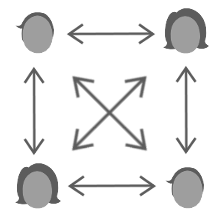
\includegraphics[scale=0.75]{real_network}
\caption{The relations between the speakers of a real sociolect}
\end{figure} 

However, the speakers of the variety used for this experiments are related in this way:

\begin{figure}[H] \centering
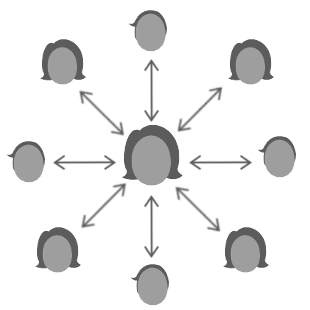
\includegraphics[scale=0.75]{sloppy_network}
\caption{The relations between the speakers in the sociolect model}
\end{figure} 

Instead of the language variety of a group of people, what is used here is more like the language used around a particular person. Although the effects of using a real sociolect model might be an interesting topic for future research, I have chosen not investigate it here, because my expectation is that it will not improve the results. Namely, a 'natural' sociolect model can only predict what a group of people will say, but it will (almost) always be one person that will be formulating the language. In other words, unless a whole group of people is writing, it is probably a better idea to use the language specific to the author.


Furthermore, the possible points of critique I formulated in the previous section (Twitter language is no real language, Twitter users are not representative of the whole population) can also be extended to this experiment: social relations as visible on Twitter are likely to be only a fraction of the real the social relations of a particular person, and might also be a misleading representation of it. For instance, people who never speak to eachother in real life might talk a lot on Twitter, and vice versa. Although this is a valid argument, I believe this only strengthens my point: if using only a noisy fraction of somebody's social relations already leads to significant results, I imagine the results will be even better when it would be possible to capture the social relations better.

\subsection{Overview}
After having discovered which algorithm provides the best results in chapter \ref{algorithm}, in this chapter the language model was investigated. The most important finding is that using idiolect models leads to the most keystrokes saved by far. Idiolect models fail when the user writes about something he/she has not written about before, but these situations can be covered by either by the recency buffer, which learns from the text as the user is writing it and thus has information on what the text is about, or by the general language model, which has general information about the language the user is using, and thus can do general predictions as long as the things the user is saying are not too unusual in that language. 

These findings were also clearly visible when replicated with 100 Twitter feeds as idiolects. Interestingly they were not equally strong for every speaker; apparently, for some speakers language is easier to predict than for others. Furthermore, because people who are in some way related tend to speak alike, it was also tested whether adding tweets of the people these 100 Twitter users communicated with often could increase the results. This turned out to be the case. Here again, this worked better for some users than for others. The best result that was achieved was a \textbf{56\% CKS} and a \textbf{58\% SKKS}.

To summarize this all in one statement: to save the most keystrokes, it is best to use language as close as possible to the user of the word prediction system.










\section{Conclusion} \label{conclusion}
In this thesis, I have described the workings of my word prediction system \emph{Soothsayer}. Furthermore, I hope to have made clear a number of things:

\begin{enumerate}
\item Word prediction and idiolects are a golden combination.
\item When building a word prediction system, concentrating on either the algorithm or the language model alone is not enough.
\item What works well for one speaker, might not necessarily work for another.
\item The fact that people speak like the people around them can also be useful to word prediction.
\end{enumerate}

From here, there are a number of ways this research could go. One could, for example, try to answer the questions these conclusions inevitably raise. What causes the differences between speakers? Can we, on the basis of texts the user wrote earlier, predict what will work and what will not? Or could we adapt the system on the fly, so that it can be most useful to a particular user? And what would be a practical implication of the discoveries related to sociolects? Would a social media plugin to share language models between friends work? 

Another group of questions that can still be answered can be found when the limitations I set at the beginning of this thesis are removed. What would be the effects of predicting more words at the same time? What are Soothsayer's pros and cons if we focus on one specific domain of word prediction, like query completion?

Whatever the answers to these questions may be, they will only improve (or clear up) what we have so far: well-performing, state-of-the-art word prediction software, freely available on the internet for everyone to change, improve and most important of all: use. Soothsayer can be used however you want: as standalone software wrapped inside other software, from the cloud with its HTTP-server mode, or even as a Python module. I really hope this means it will find its way into a practical application someday, so it can do what is was built to do 'for real': guessing what somebody is going to w$|$\emph{rite}.

\section{Acknowledgements/dankwoord}

% Eenzaam, 'gevecht tussen man en computer'. Bedank Hannah, Iris, Kobie, Ali en Florian.
% Véronique onderwerp, en Lieke voor idiolect ipv ideolect.
% Maarten, Florian en Bouke voor de vele dingen programmeren.
% Antal: mails. Tegelijkertijd waren we met nog veel andere dingen bezig. Veel baantjes bezorgd.
% Is ook afsluiting van mijn studententijd. Helen, als tutor en zo ongeveer driekwart van mijn cursussen. G&C
% Hilde: laat Soothsayer spreken

\bibliography{thesisbib}{}
\bibliographystyle{apacite}

\end{document}

%TODO
% Consistent zijn in model, corpus, training material, text, idiolect vs personal... bijv. bij modules heet het 'model', in de resultaten 'training material'
% Statistiek: assumpties checken
